\documentclass[12pt]{article} % Tipo de documento

% Paquetes básicos
\usepackage[utf8]{inputenc}   % Permite caracteres en UTF-8
\usepackage[T1]{fontenc}      % Codificación de fuente
\usepackage[spanish]{babel}   
\usepackage{lmodern}          
\usepackage{geometry}         
\usepackage{graphicx}        
\usepackage{amsmath, amssymb} 
\usepackage{setspace}         
\usepackage{hyperref}        
\usepackage{graphicx}
\usepackage{booktabs}
\usepackage{float}

% Configuración de márgenes y espaciado
\geometry{a4paper, margin=2.5cm}
\setstretch{1.2}

% Datos del título
\title{Nf-L e IL-6 como predictores de supervivencia y función motora en pacientes con ELA}
\author{Daniel Camacho Montaño}
\date{30 de diciembre de 2024}

\begin{document}

\maketitle 
\newpage
\begin{abstract}
El presente informe analiza la relación entre biomarcadores sanguíneos y características clínicas con la progresión funcional y la supervivencia de pacientes con esclerosis lateral amiotrófica (ELA), utilizando el conjunto de datos \texttt{ela\_allBiomarkers.csv} de 128 pacientes distribuidos en tres cohortes. Se evaluó la capacidad predictiva de un panel de biomarcadores (Nf-L, CRP e IL-6) sobre la supervivencia a 36 meses mediante regresión logística, observándose que niveles elevados de Nf-L e IL-6 se asocian con menor probabilidad de supervivencia, y que el sitio de inicio de la enfermedad influye significativamente en el pronóstico. La inclusión de IL-6 mejora notablemente la capacidad predictiva del modelo, con un pseudo $R^2$ de McFadden de 0.201 y un desempeño moderado en la cohorte de validación externa ($accuracy = 0.727$, $Kappa = 0.455$). 

Asimismo, se estudió la relación entre Nf-L y la puntuación basal de la Escala Revisada de Calificación Funcional de la ELA (ALSFRS-R) mediante modelos de regresión lineal ordinarios y robustos. Se confirmó que niveles más altos de Nf-L se asocian con puntuaciones funcionales más bajas, mientras que la interacción entre sexo y edad resulta significativa únicamente en mujeres. La eliminación de observaciones influyentes mejoró la estabilidad del modelo y aumentó el coeficiente de determinación ajustado de 0.1688 a 0.2689. 

Finalmente, se evaluó la capacidad predictiva de las variables sobre ALSFRS-R utilizando modelos OLS, stepwise, PLS y LASSO. Los resultados destacaron a Nf-L y el sitio de inicio como principales predictores del deterioro funcional. La comparación de los modelos mediante RMSE en la cohorte de validación mostró que el modelo LASSO proporciona el ajuste más eficiente ($RMSE = 5.207$), seleccionando únicamente Nf-L e IL-6 como variables activas. Estos hallazgos subrayan la relevancia de los biomarcadores Nf-L e IL-6 en la caracterización del pronóstico y la progresión funcional de pacientes con ELA, ofreciendo herramientas útiles para la estratificación de riesgo y el seguimiento clínico.
\end{abstract}
\newpage
\begin{abstract}
This report analyzes the relationship between blood biomarkers and clinical characteristics with functional progression and survival in patients with amyotrophic lateral sclerosis (ALS), using the \texttt{ela\_allBiomarkers.csv} dataset comprising 128 patients across three cohorts. The predictive value of a panel of biomarkers (Nf-L, CRP, and IL-6) for 36-month survival was assessed using logistic regression, showing that elevated levels of Nf-L and IL-6 are associated with lower survival probability, while disease onset site significantly influences prognosis. Inclusion of IL-6 substantially improved model performance, with a McFadden pseudo $R^2$ of 0.201 and moderate predictive accuracy in the external validation cohort ($accuracy = 0.727$, $Kappa = 0.455$).

Additionally, the relationship between Nf-L and baseline ALS Functional Rating Scale-Revised (ALSFRS-R) scores was evaluated using ordinary and robust linear regression models. Higher Nf-L levels were associated with lower functional scores, and the age-sex interaction was significant only in women. Exclusion of influential observations improved model stability and increased the adjusted $R^2$ from 0.1688 to 0.2689.

Finally, predictive performance for ALSFRS-R was examined using OLS, stepwise, PLS, and LASSO regression models. Nf-L and onset site emerged as the primary predictors of functional decline. Model comparison via RMSE on the validation cohort indicated that LASSO provided the most efficient fit ($RMSE = 5.207$), selecting only Nf-L and IL-6 as active predictors. These findings highlight the importance of Nf-L and IL-6 in prognostic assessment and functional monitoring in ALS patients, offering valuable tools for risk stratification and clinical follow-up.
\end{abstract}


\newpage
\tableofcontents 
\newpage

\section{Análisis del conjunto de biomarcadores en pacientes con ELA}

El presente informe analiza el conjunto de datos \texttt{ela\_allBiomarkers.csv}, utilizado en el estudio de Simon Witzel et al.\ (2021), cuyo objetivo fue evaluar si un panel de biomarcadores sanguíneos puede contribuir a predecir la progresión de la esclerosis lateral amiotrófica (ELA). Para ello, los autores incluyeron 128 pacientes diagnosticados con ELA, procedentes de tres cohortes prospectivas: una cohorte de desarrollo del modelo (\textit{DevCohort}) y dos cohortes adicionales empleadas para su validación externa (\textit{ValCohort1} y \textit{ValCohort2}).

Los datos fueron cargados en R mediante lectura directa del archivo CSV, observándose inicialmente que no existían valores ausentes y que el conjunto estaba formado por 11 variables: tres categóricas (\texttt{cohort}, \texttt{onset}, \texttt{sex}) y siete continuas. La variable \texttt{patient} no se consideró un factor relevante, ya que únicamente identificaba a los sujetos (p1--p128). Para asegurar una correcta manipulación estadística, las variables categóricas fueron convertidas explícitamente a factores mediante la función \texttt{as.factor()}.

Posteriormente se verificó la estructura interna del conjunto de datos para confirmar la correcta codificación de las variables.

\begin{verbatim}
    'data.frame':	128 obs. of  11 variables:
 $ patient         : chr  "p1" "p2" "p3" "p4" ...
 $ cohort          : Factor w/ 3 levels "DevCohort","ValCohort1",..: 1 1 1 1 1 1 1 1 1 1 ...
 $ onset           : Factor w/ 2 levels "bulbar","spinal": 2 2 2 2 2 2 2 2 2 2 ...
 $ sex             : Factor w/ 2 levels "female","male": 2 2 2 1 2 2 2 2 1 2 ...
 $ age             : int  51 75 57 62 72 37 75 72 46 66 ...
 $ BMI_baseline    : num  32.8 24.8 23.5 23.3 28 ...
 $ ALSFRSR_baseline: num  33 36 45 27 32 44 46 45 37 43 ...
 $ NfL_baseline    : int  19 194 60 230 80 78 57 155 143 46 ...
 $ CRP_baseline    : num  43.2 30.9 59.2 12.3 50.5 ...
 $ IL6_baseline    : num  83.6 89.2 50 53.1 20.8 ...
 $ months_survived : num  28 26 40 27 69 34 63 26 39 24 ...
\end{verbatim}

El estudio se centra particularmente en tres biomarcadores medidos en sangre: \texttt{Nf-L}, \texttt{CRP} e \texttt{IL-6}. El neurofilamento ligero (Nf-L) es un componente estructural de los axones neuronales cuya presencia en fluidos corporales aumenta ante daño axonal, por lo que constituye un biomarcador ampliamente utilizado en enfermedades neurodegenerativas. Por su parte, CRP e IL-6 son moléculas relacionadas con la respuesta inflamatoria: la proteína C-reactiva (CRP) es sintetizada en el hígado y actúa como marcador general de inflamación sistémica, mientras que la interleucina-6 (IL-6) es una citoquina clave en la regulación de la respuesta inmune y se asocia frecuentemente a procesos inflamatorios y neuroinflamatorios presentes en pacientes con ELA.

Además de los biomarcadores sanguíneos, el conjunto de datos incluye información clínica relevante sobre los pacientes, como el sitio de inicio de la enfermedad (\texttt{onset}), el sexo (\texttt{sex}), la edad, el índice de masa corporal al inicio del estudio (\texttt{BMI\_baseline}), el tiempo de supervivencia en meses y la puntuación en la Escala Revisada de Calificación Funcional de la ELA (ALSFRS-R). Esta última constituye una medida fundamental del estado funcional del paciente, donde puntuaciones más altas indican menor impacto de la enfermedad en las actividades de la vida diaria.

El análisis realizado en este informe se basa en esta estructura de datos, permitiendo explorar la relación entre los biomarcadores sanguíneos, las características clínicas de los pacientes y la progresión de la enfermedad en las diferentes cohortes incluidas.

\subsection{Modelo de regresión logística para la predicción de supervivencia a 36 meses}

Para evaluar los determinantes de la supervivencia a los 36 meses desde el inicio de la enfermedad, se generó una variable binaria a partir de \texttt{months\_survived}, de modo que la nueva variable \texttt{survived} toma el valor 1 cuando el paciente alcanza los 36 meses de supervivencia y 0 en caso contrario. A partir de esta variable, la tasa de supervivencia se estimó mediante su promedio, obteniéndose que el 44.53\% de los pacientes incluidos en el estudio superaron dicho umbral temporal.

Con el objetivo de construir un modelo predictivo, el análisis se restringió a las cohortes \textit{DevCohort} y \textit{ValCohort1}. Sobre este subconjunto se ajustó un modelo de regresión logística, incluyendo como predictores la edad, el sexo, el índice de masa corporal basal, el sitio de inicio de la enfermedad (\textit{onset}) y los biomarcadores séricos Nf-L, CRP e IL-6.

El modelo ajustado proporcionó las estimaciones resumidas en la Tabla~\ref{tab:logit_coeff}, donde se observa que los predictores con significancia estadística fueron el sitio de inicio de la enfermedad, Nf-L e IL-6. Estos últimos mostraron efectos negativos sobre la probabilidad de supervivencia, coherentes con su papel como marcadores de daño axonal e inflamación sistémica, respectivamente. En contraste, las variables demográficas (edad, sexo) y antropométricas (IMC), así como CRP, no mostraron una asociación significativa con la supervivencia a 36 meses.

\begin{table}[h!]
\centering
\caption{Coeficientes del modelo de regresión logística para la predicción de supervivencia a 36 meses.}
\label{tab:logit_coeff}
\begin{tabular}{lrrrr}
\hline
\textbf{Variable} & \textbf{Estimación} & \textbf{Error estándar} & \textbf{Estadístico Z} & \textbf{p-valor} \\
\hline
Intercept      &  0.5817 & 0.4056 &  1.4340 & 0.1552 \\
Edad           & -0.0019 & 0.0040 & -0.4765 & 0.6349 \\
Sexo (varón)   &  0.1048 & 0.0885 &  1.1841 & 0.2396 \\
IMC            &  0.0130 & 0.0114 &  1.1413 & 0.2569 \\
Inicio espinal &  0.1942 & 0.1053 &  1.8443 & 0.0685$^\cdot$ \\
Nf-L           & -0.0008 & 0.0004 & -2.0684 & 0.0416$^\ast$ \\
CRP            & -0.0013 & 0.0015 & -0.8743 & 0.3844 \\
IL-6           & -0.0086 & 0.0018 & -4.8096 & $<\,0.001^{\ast\ast\ast}$ \\
\hline
\end{tabular}
\end{table}

La evaluación de la significancia de los coeficientes se realizó mediante el estadístico Z, que bajo la hipótesis nula de ausencia de efecto sigue una distribución normal estándar. Para un nivel de significancia del 10\%, los valores críticos se sitúan en el intervalo aproximado $[-1.645,\, 1.645]$. Los estadísticos Z obtenidos para cada predictor se muestran en la tabla anterior y revelan que únicamente IL-6, Nf-L y el sitio de inicio superan estos umbrales. La información adicional proporcionada por la salida del modelo muestra que IL-6 es el predictor con mayor magnitud de efecto y mayor evidencia estadística.

En conjunto, estos resultados indican que tanto el daño neuronal (reflejado por los niveles de Nf-L) como la intensidad del proceso inflamatorio (capturada por IL-6) desempeñan un papel determinante en la supervivencia a medio plazo. Asimismo, el sitio anatómico de inicio de la enfermedad también aporta información relevante en la predicción del desenlace. Por el contrario, las características demográficas y clínicas basales no mostraron una influencia significativa en este análisis.

\subsection{Interpretación de los coeficientes y análisis del modelo reducido}

La interpretación del modelo de regresión logística ajustado permite evaluar cómo influyen los biomarcadores y las características clínicas en la probabilidad de que un paciente sobreviva al menos 36 meses desde el inicio de la enfermedad. Dado que la variable respuesta toma el valor 1 para los individuos que superan este umbral temporal, los coeficientes positivos indican una mayor probabilidad de supervivencia, mientras que los coeficientes negativos reflejan un pronóstico desfavorable.

En este contexto, los biomarcadores Nf-L e IL-6 se identifican como predictores especialmente relevantes, ambos con coeficientes negativos y estadísticamente significativos. Este patrón es consistente con la evidencia fisiopatológica: concentraciones elevadas de Nf-L implican un mayor grado de daño axonal, mientras que IL-6 es un marcador de inflamación sistémica asociado a procesos neurodegenerativos más agresivos. Los signos negativos de estos coeficientes sugieren que niveles incrementados de estos biomarcadores se relacionan con una menor probabilidad de supervivencia a medio plazo.

Asimismo, el inicio espinal de la enfermedad mostró un efecto positivo sobre la probabilidad de supervivencia, indicando que los pacientes con inicio espinal presentan un pronóstico más favorable en comparación con el inicio bulbar, como se ha documentado previamente en la literatura clínica.

Con el objetivo de evaluar la estabilidad del modelo y la contribución específica de IL-6, se ajustó un modelo reducido en el que se excluyó dicho biomarcador. En esta nueva especificación, Nf-L mantuvo su significancia y el efecto del inicio espinal se incrementó, alcanzando significancia al 5\%. Esto sugiere que parte de la variabilidad explicada por IL-6 se redistribuye entre las covariables restantes al eliminar este predictor, modificando la magnitud relativa de sus asociaciones.

La comparación formal entre el modelo completo y el modelo reducido se llevó a cabo mediante un análisis de la desviancia, que evalúa si la inclusión del biomarcador IL-6 mejora significativamente la capacidad predictiva. Los modelos considerados fueron: el modelo reducido, que incluye únicamente los predictores clínicos y los biomarcadores Nf-L y CRP, y el modelo completo, que añade IL-6 como covariable adicional. La tabla siguiente resume los resultados del contraste:

\begin{verbatim}
Analysis of Deviance Table

Model 1: survived ~ age + sex + BMI_baseline + onset + NfL_baseline 
        + CRP_baseline
Model 2: survived ~ age + sex + BMI_baseline + onset + NfL_baseline 
        + CRP_baseline + IL6_baseline

  Resid. Df Resid. Dev Df Deviance  Pr(>Chi)    
1        88     17.966                          
2        87     14.193  1   3.7736 1.512e-06 ***
\end{verbatim}

El contraste de razón de verosimilitudes muestra un valor p extremadamente pequeño, lo que indica que la reducción en la desviancia tras incluir IL-6 es altamente significativa. Dado que ambos modelos son anidados y difieren únicamente en un parámetro, este resultado permite rechazar la hipótesis nula que plantea que el coeficiente asociado a IL-6 es igual a cero. Formalmente, el contraste evalúa:

\[
H_0: \beta_{\text{IL-6}} = 0 \qquad \text{(IL-6 no aporta información adicional)}
\]
\[
H_1: \beta_{\text{IL-6}} \neq 0 \qquad \text{(IL-6 mejora el ajuste del modelo)}
\]

La evidencia empírica respalda la inclusión de IL-6 en el modelo, confirmando que este biomarcador aporta información predictiva independiente sobre la supervivencia a 36 meses. Su exclusión no solo empeora la calidad del ajuste, sino que también redistribuye la importancia relativa de los otros predictores, reforzando su relevancia como componente esencial del modelo final.

En conjunto, el análisis pone de manifiesto que los marcadores de neurodegeneración e inflamación, particularmente Nf-L e IL-6, desempeñan un papel fundamental en la caracterización del pronóstico, mientras que el tipo de inicio de la enfermedad también contribuye de manera apreciable a la explicación de la variabilidad en la supervivencia.

\subsection{Pseudo R\textsuperscript{2} de McFadden para el modelo de regresión logística}

En los modelos de regresión lineal, el coeficiente de determinación $R^2$ resume la proporción de varianza en la variable dependiente que se explica mediante las variables predictoras. Sin embargo, en modelos lineales generalizados, como la regresión logística, la variable dependiente no es continua, por lo que el cálculo directo de $R^2$ no es adecuado. Una alternativa ampliamente utilizada es el \textit{pseudo} $R^2$ de McFadden, definido a partir de las log-verosimilitudes del modelo nulo (sin predictores) y del modelo estimado:

\[
R^2_{\text{McFadden}} = 1 - \frac{\log L(\text{modelo completo})}{\log L(\text{modelo nulo})}.
\]

Para calcular este índice se obtuvieron las log-verosimilitudes de los modelos completo y reducido, y se aplicó la fórmula anterior. El valor obtenido, $R^2_{\text{McFadden}} = 0.20109$, indica que el modelo explica aproximadamente un 20\% de la variabilidad relativa en la supervivencia a 36 meses. Este resultado sugiere que el poder explicativo del modelo es moderado-bajo, lo que podría deberse a la inclusión de predictores no relevantes, ya que de las seis variables consideradas solo tres resultaron significativas.

No obstante, el pseudo $R^2$ de McFadden debe interpretarse como una medida de ajuste relativo y en conjunto con otras métricas, como análisis de residuos, validación cruzada o comparación con modelos alternativos, para obtener una evaluación más completa de la capacidad predictiva del modelo.

\subsection{Evaluación de la capacidad diagnóstica del modelo}

La capacidad diagnóstica del modelo de regresión logística se evaluó mediante predicciones sobre la cohorte de validación independiente \textit{ValCohort2}. A partir del modelo ajustado con las cohortes de desarrollo y primera validación (\textit{DevCohort} y \textit{ValCohort1}), se calcularon las probabilidades predichas de supervivencia a 36 meses para cada paciente de \textit{ValCohort2}. Estas probabilidades se transformaron en clases binarias utilizando un umbral de 0.5, de modo que un valor predicho mayor o igual a 0.5 se consideró como supervivencia, y valores menores como no supervivencia:

La comparación entre las predicciones del modelo y los resultados observados se realizó mediante una matriz de confusión, utilizando la función \texttt{confusionMatrix()} del paquete \texttt{caret}. 

El resultado de la matriz de confusión se resume a continuación:

\begin{verbatim}
          Reference
Prediction  0  1
         0 12  4
         1  5 12
                                          
               Accuracy : 0.7273         
                 95% CI : (0.5448, 0.867)
    No Information Rate : 0.5152         
    P-Value [Acc > NIR] : 0.01081        
                                          
                  Kappa : 0.455          
                                          
 Mcnemar's Test P-Value : 1.00000        
                                          
            Sensitivity : 0.7059         
            Specificity : 0.7500         
         Pos Pred Value : 0.7500         
         Neg Pred Value : 0.7059         
             Prevalence : 0.5152         
         Detection Rate : 0.3636         
   Detection Prevalence : 0.4848         
      Balanced Accuracy : 0.7279         
                                          
       'Positive' Class : 0
\end{verbatim}

El análisis indica que el modelo presenta una sensibilidad del 70.6\%, lo que refleja su capacidad para identificar correctamente a los pacientes que efectivamente sobreviven 36 meses. La especificidad es del 75\%, indicando que el modelo también distingue razonablemente bien a los pacientes que no alcanzan este umbral de supervivencia. 

El índice Kappa, que ajusta la concordancia entre predicciones y observaciones reales por el acuerdo esperado al azar, es de 0.455, mostrando un grado de concordancia moderado. Por otra parte, el valor predictivo positivo alcanza el 75\%, lo que significa que de cada 100 pacientes clasificados como sobrevivientes, 75 efectivamente superaron los 36 meses.

En conclusión, el modelo es útil para la predicción de supervivencia a 36 meses, aunque existen márgenes de mejora en términos de precisión y concordancia, lo que sugiere que futuras refinaciones del modelo podrían incrementar su capacidad diagnóstica.

\section{Análisis de la relación entre Nf-L y la puntuación basal de ALSFRS-R}

Se analizó la asociación entre el biomarcador Nf-L y la puntuación basal de la Escala Revisada de Calificación Funcional de la ELA (ALSFRS-R), utilizando los datos combinados de las cohortes \textit{DevCohort} y \textit{ValCohort1}. Para ello, se ajustó un modelo de regresión lineal mediante Mínimos Cuadrados Ordinarios (OLS), considerando como covariables el sitio de inicio de la enfermedad (\textit{onset}), edad y sexo, e incluyendo una interacción entre edad y sexo para capturar posibles diferencias en el efecto de la edad según el sexo:

\[
\text{ALSFRSR} = \beta_0 + \beta_1 \text{Nf-L} + \beta_2 \text{onset} + \beta_3 \text{sex} + \beta_4 \text{age} + \beta_5 (\text{sex} \times \text{age}) + \varepsilon
\]

El ajuste del modelo se realizó con la función \texttt{lm()} en R, obteniéndose los resultados resumidos en la Tabla~\ref{tab:lm_ALSFRSR}.

\begin{table}[h!]
\centering
\caption{Coeficientes del modelo de regresión lineal para la puntuación basal de ALSFRS-R.}
\label{tab:lm_ALSFRSR}
\begin{tabular}{lrrrr}
\hline
\textbf{Variable} & \textbf{Estimación} & \textbf{Error estándar} & \textbf{t} & \textbf{p-valor} \\
\hline
Intercept      & 54.1624 & 6.6585 & 8.134  & $2.3 \times 10^{-12}$ *** \\
Nf-L           & -0.0212 & 0.0053 & -3.975 & 0.000143 *** \\
Inicio espinal & -3.2886 & 1.5937 & -2.063 & 0.04198 * \\
Sexo (varón)   & -12.0040 & 7.7593 & -1.547 & 0.1254 \\
Edad           & -0.1848 & 0.1038 & -1.781 & 0.0783 . \\
Sexo $\times$ Edad & 0.2198 & 0.1257 & 1.748 & 0.0838 . \\
\hline
\end{tabular}
\end{table}

Los resultados muestran que los niveles de Nf-L y el inicio espinal son predictores significativos de la puntuación basal de ALSFRS-R al nivel del 5\%, ambos con efectos negativos: niveles más altos de Nf-L se asocian con puntuaciones más bajas, reflejando un mayor deterioro funcional, mientras que los pacientes con inicio espinal presentan puntuaciones iniciales inferiores a los de inicio bulbar.

La interacción entre sexo y edad no alcanza significancia al 5\%, aunque evidencia al 10\% sugiere que el efecto de la edad sobre la puntuación ALSFRS-R podría diferir entre hombres y mujeres.

El coeficiente de determinación ajustado ($R^2_\text{adj} = 0.1688$) indica que el modelo explica aproximadamente el 21.3\% de la variabilidad de la puntuación basal. A pesar de este valor relativamente bajo, el estadístico F global es significativo ($p = 0.0006$), confirmando que al menos uno de los predictores contribuye de manera relevante a la explicación de la variable respuesta.

\subsection{Contrastes de hipótesis sobre los determinantes de ALSFRS-R}

A partir del modelo de regresión lineal ajustado para la puntuación basal de ALSFRS-R, se evaluaron hipótesis específicas sobre la significancia de los predictores principales. Se asumió un nivel de significancia $\alpha = 0.10$ para todos los contrastes.

\subsubsection*{Análisis del efecto del biomarcador Nf-L}

Se planteó la hipótesis de que Nf-L tiene un efecto significativo sobre la puntuación ALSFRS-R:

\[
H_0: \beta_{\text{Nf-L}} = 0 \qquad \text{vs.} \qquad H_1: \beta_{\text{Nf-L}} \neq 0
\]

El coeficiente estimado para Nf-L fue $\hat{\beta}_{\text{Nf-L}} = -0.0212$ con $p = 0.000143$. Dado que el p-valor es menor que 0.10, se rechaza la hipótesis nula, concluyendo que Nf-L es un predictor significativo de la puntuación basal de ALSFRS-R, con efecto negativo: niveles más altos de Nf-L se asocian con puntuaciones funcionales más bajas.

\subsubsection*{Análisis del efecto de la edad en mujeres}

Para evaluar el efecto de la edad en el grupo femenino, se ajustó el modelo únicamente sobre las mujeres, considerando la edad junto con Nf-L y el sitio de inicio. La hipótesis formulada fue:

\[
H_0: \beta_{\text{edad}} = 0 \qquad \text{vs.} \qquad H_1: \beta_{\text{edad}} \neq 0
\]

El coeficiente estimado fue $\hat{\beta}_{\text{edad}} = -0.188$ con $p = 0.089$, lo que indica significancia al nivel del 10\%, pero no al 5\%. Por tanto, se rechaza la hipótesis nula al 10\% y se concluye que la edad afecta significativamente la puntuación ALSFRS-R en mujeres, mostrando una tendencia negativa: puntuaciones más bajas con mayor edad.

\subsubsection*{Análisis del efecto de la edad en hombres}

De manera análoga, se evaluó el efecto de la edad en el grupo masculino:

\[
H_0: \beta_{\text{edad}} = 0 \qquad \text{vs.} \qquad H_1: \beta_{\text{edad}} \neq 0
\]

En este caso, el coeficiente estimado fue $\hat{\beta}_{\text{edad}} = 0.034$ con $p = 0.650$, valor que no permite rechazar la hipótesis nula. Esto indica que en hombres la edad no tiene un efecto significativo sobre la puntuación basal de ALSFRS-R.

\subsubsection*{Interpretación general}

Estos resultados muestran que la interacción entre sexo y edad es relevante únicamente para las mujeres, mientras que no se observa un efecto significativo en los hombres. Además, se confirma la relevancia de Nf-L como predictor negativo de la puntuación funcional basal en ambos sexos.


\subsection{Análisis de residuos y observaciones influyentes}

Para evaluar la adecuación del modelo de regresión lineal ajustado sobre la puntuación basal de ALSFRS-R, se realizó un análisis de residuos utilizando los gráficos de diagnóstico estándar. Estos incluyeron: residuos vs valores ajustados, gráfico Q-Q, escala-localización y distancia de Cook.

\begin{figure}[h!]
\centering
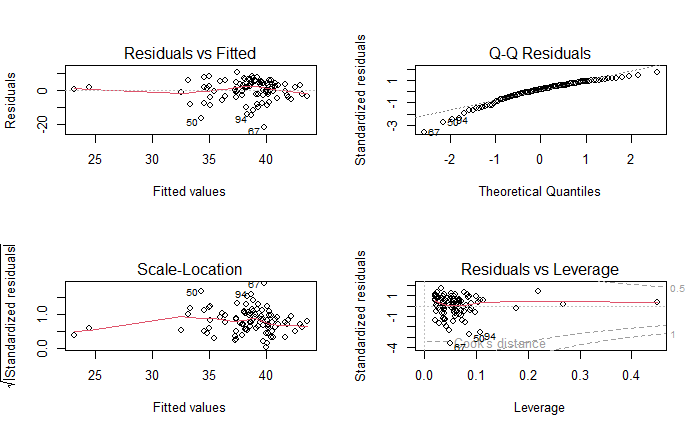
\includegraphics[width=0.8\textwidth]{residuals_diagnostics.png}
\caption{Gráficos de diagnóstico del modelo de regresión lineal: residuos vs valores ajustados, gráfico Q-Q y escala-localización.}
\label{fig:residuos_diagnostico}
\end{figure}

El gráfico Q-Q muestra que algunos puntos extremos se alejan de la distribución normal, indicando ligeras desviaciones respecto a la normalidad de los residuos. En el gráfico de residuos frente a valores ajustados se observa que los residuos no se distribuyen completamente de manera uniforme, presentando una ligera concentración hacia valores más altos. No obstante, los valores de leverage permanecen relativamente bajos, lo que sugiere que ninguna observación ejerce un apalancamiento excesivo sobre los coeficientes del modelo.

\begin{figure}[h!]
\centering
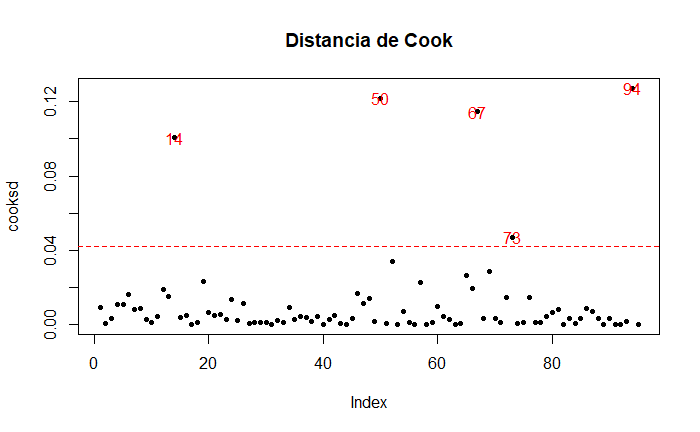
\includegraphics[width=0.8\textwidth]{000014.png}
\caption{Gráficos distancia de Cook.}
\label{fig:Cook_diagnostico}
\end{figure}

Se identificaron observaciones con alta influencia mediante la distancia de Cook. Cinco observaciones (14, 50, 67, 73 y 94) superan el umbral de referencia, indicando que podrían ser influyentes en el ajuste. A pesar de esta influencia relativa, sus valores no alcanzan magnitudes extremas, lo que sugiere que el modelo conserva estabilidad global.

En conjunto, estos análisis corroboran que el modelo ajusta razonablemente los datos, aunque la presencia de algunas observaciones influyentes podría justificar un análisis de sensibilidad o la consideración de modelos robustos como complemento.


\subsection{Modelo robusto y ajuste tras eliminar observaciones problemáticas}

Dado que el análisis de residuos previo identificó observaciones influyentes, se ajustó una versión robusta del modelo de regresión lineal utilizando el método de Huber para minimizar el impacto de estas observaciones extremas. Este enfoque permite ponderar las observaciones de manera que aquellas con valores atípicos o altamente influyentes contribuyan menos al ajuste del modelo.

En el modelo robusto, se identificaron 18 observaciones con pesos inferiores a 1, indicando que su influencia se redujo durante el ajuste. Entre ellas, cinco coincidían con las observaciones problemáticas detectadas en el modelo OLS (14, 50, 67, 73 y 94), lo que confirma que estas observaciones son especialmente influyentes y deben ser examinadas con detalle. Las demás observaciones con peso reducido reflejan diferencias en la sensibilidad de los métodos OLS y robusto frente a valores extremos.

Para evaluar el impacto de estas observaciones en el ajuste del modelo, se construyó un nuevo conjunto de datos excluyendo las cinco observaciones influyentes y se ajustó nuevamente el modelo de regresión lineal. La comparación de los coeficientes y del ajuste general mostró que el coeficiente de Nf-L permaneció significativo y negativo, mientras que la interacción entre sexo y edad dejó de ser significativa al 10\%, y la variable edad conservó su significancia al 10\%. Además, la desviación estándar residual disminuyó, indicando un ajuste más preciso, y el coeficiente de determinación ajustado aumentó de 0.1688 a 0.2689, reflejando que el modelo explica una mayor proporción de la variabilidad de la puntuación basal de ALSFRS-R.

\begin{table}[h!]
\centering
\caption{Comparación de criterios de información entre el modelo original y el modelo ajustado sin observaciones problemáticas.}
\label{tab:aic_bic_comparison}
\begin{tabular}{lrr}
\hline
\textbf{Modelo} & \textbf{AIC} & \textbf{BIC} \\
\hline
Original & 622.99 & 640.86 \\
Sin observaciones problemáticas & 551.20 & 568.70 \\
\hline
\end{tabular}
\end{table}

La comparación de los criterios de información AIC y BIC (Tabla~\ref{tab:aic_bic_comparison}) confirma que el modelo sin las observaciones problemáticas es preferible: presenta valores de AIC y BIC notablemente más bajos, lo que indica un ajuste más eficiente y menos afectado por valores extremos. Estos resultados sugieren que la eliminación de las observaciones más influyentes mejora la estabilidad del modelo y la interpretación de los coeficientes, especialmente para la variable Nf-L y la interacción entre sexo y edad.

\subsection{Comparación de resultados entre modelos OLS y robusto}

Se comparan los resultados de los coeficientes estimados mediante regresión lineal OLS (sin observaciones problemáticas) y regresión robusta (método Huber) para evaluar la consistencia de la significancia de los predictores y la fiabilidad de los modelos.

\begin{table}[h!]
\centering
\caption{Coeficientes estimados y estadísticos $t$ para los modelos OLS y robusto}
\label{tab:coef_comparison}
\begin{tabular}{lcccccc}
\hline
\multirow{2}{*}{Variable} & \multicolumn{3}{c}{OLS limpio} & \multicolumn{3}{c}{Robusto (Huber)} \\
\cline{2-7}
 & Estimación & Error std & $t$ & Estimación & Error std & $t$ \\
\hline
Intercept & 51.826 & 5.849 & 8.860 & 52.100 & 5.995 & 8.691 \\
Nf-L & -0.0211 & 0.0043 & -4.861 & -0.0212 & 0.0048 & -4.421 \\
Onset espinal & -1.911 & 1.303 & -1.467 & -2.464 & 1.435 & -1.717 \\
Sexo (varón) & -7.038 & 6.888 & -1.022 & -8.251 & 6.986 & -1.181 \\
Edad & -0.159 & 0.095 & -1.674 & -0.151 & 0.093 & -1.617 \\
Sexo $\times$ Edad & 0.149 & 0.113 & 1.317 & 0.162 & 0.113 & 1.429 \\
\hline
\end{tabular}
\end{table}

Se puede observar que Nf-L mantiene una asociación negativa significativa en ambos modelos, mientras que otras variables como edad o el sitio de inicio muestran diferencias en su significancia dependiendo del método de ajuste.

\begin{table}[h!]
\centering
\caption{Indicadores de ajuste global de los modelos OLS y robusto}
\label{tab:model_fit}
\begin{tabular}{lcc}
\hline
Modelo & $R^2_\text{adj}$ & Residual Std. Error \\
\hline
OLS limpio & 0.2689 & 4.953 \\
Robusto (Huber) & - & 5.061 \\
\hline
\end{tabular}
\end{table}

El modelo OLS presenta un $R^2_\text{adj}$ ligeramente mayor y más variables significativas, mientras que el modelo robusto ofrece mayor protección frente a observaciones influyentes, proporcionando un ajuste más estable y confiable para la inferencia estadística.

\section{Capacidad predictiva de las variables para ALSFRS-R}

Se evaluó la capacidad de predicción de distintas variables sobre la puntuación basal de la Escala Revisada de Calificación Funcional de la ELA (ALSFRS-R), utilizando los datos de las cohortes \textit{DevCohort} y \textit{ValCohort1} (\texttt{cohort\_data}). Para garantizar la reproducibilidad de los resultados, se fijó la semilla con \texttt{set.seed(123)}.

Se ajustó un modelo de regresión lineal OLS considerando como variables predictoras la edad, sexo (convertido a variable numérica), índice de masa corporal (BMI), sitio de inicio de la enfermedad (\textit{onset}), niveles basales de Nf-L, CRP e IL-6:

\[
\text{ALSFRSR} = \beta_0 + \beta_1 \text{age} + \beta_2 \text{sex} + \beta_3 \text{BMI} + \beta_4 \text{onset} + \beta_5 \text{Nf-L} + \beta_6 \text{CRP} + \beta_7 \text{IL6} + \varepsilon
\]

El resumen del ajuste se presenta en la Tabla~\ref{tab:ols_predictive}.

\begin{table}[h!]
\centering
\caption{Coeficientes estimados del modelo OLS para ALSFRS-R}
\label{tab:ols_predictive}
\begin{tabular}{lrrrr}
\hline
\textbf{Variable} & \textbf{Estimación} & \textbf{Error estándar} & \textbf{t} & \textbf{p-valor} \\
\hline
Intercept      & 41.852 & 6.586 & 6.355 & $9.28\times10^{-9}$ *** \\
Edad           & -0.041 & 0.062 & -0.665 & 0.508 \\
Sexo           & 1.065 & 1.378 & 0.773 & 0.442 \\
BMI            & 0.030 & 0.177 & 0.168 & 0.867 \\
Inicio espinal & -2.660 & 1.639 & -1.623 & 0.108 \\
Nf-L           & -0.023 & 0.006 & -3.917 & 0.000178 *** \\
CRP            & 0.002 & 0.024 & 0.101 & 0.920 \\
IL-6           & 0.032 & 0.028 & 1.161 & 0.249 \\
\hline
\end{tabular}
\end{table}

Los resultados indican que únicamente Nf-L y el intercepto son estadísticamente significativos al nivel del 5\%, mostrando un efecto negativo: niveles más altos de Nf-L se asocian con puntuaciones más bajas de ALSFRS-R, independientemente de las demás variables consideradas. 

El coeficiente de determinación del modelo ($R^2 = 0.1995$, $R^2_\text{adj} = 0.1351$) es relativamente bajo, indicando que aproximadamente el 20\% de la variabilidad en la puntuación basal de ALSFRS-R se explica por las variables incluidas. No obstante, el estadístico F global es significativo ($p = 0.00578$), lo que confirma que al menos uno de los predictores contribuye de manera relevante a la explicación de la variable respuesta. 

Estos hallazgos destacan la relevancia de Nf-L como biomarcador potencialmente clave para la evaluación de la progresión funcional en pacientes con ELA.

\subsection{Evaluación de multicolinealidad}

Se evaluó la posible multicolinealidad entre las variables predictoras del modelo OLS ajustado para ALSFRS-R mediante el cálculo del \emph{Factor de Inflación de la Varianza} (VIF), utilizando el paquete \texttt{car}. Los valores obtenidos se muestran en la Tabla~\ref{tab:vif}.

\begin{table}[h!]
\centering
\caption{Valores del Factor de Inflación de la Varianza (VIF) para las variables regresoras}
\label{tab:vif}
\begin{tabular}{lr}
\hline
\textbf{Variable} & \textbf{VIF} \\
\hline
Edad             & 1.062 \\
Sexo             & 1.074 \\
BMI              & 1.008 \\
Inicio espinal   & 1.219 \\
Nf-L             & 1.372 \\
CRP              & 1.173 \\
IL-6             & 1.117 \\
\hline
\end{tabular}
\end{table}

Los valores de VIF cercanos a 1 indican ausencia de correlación entre las variables, mientras que valores superiores a 5 evidenciarían una multicolinealidad problemática. Los resultados muestran que todas las variables presentan correlaciones moderadas y aceptables.

Como análisis complementario, se calculó la matriz de correlación entre las variables numéricas y se visualizó mediante un diagrama de círculos, usando \texttt{corrplot} (Figura~\ref{fig:corrplot}). En este gráfico, el tamaño de los círculos indica la magnitud de la correlación y la escala de color la dirección de la misma.

\begin{figure}[h!]
\centering
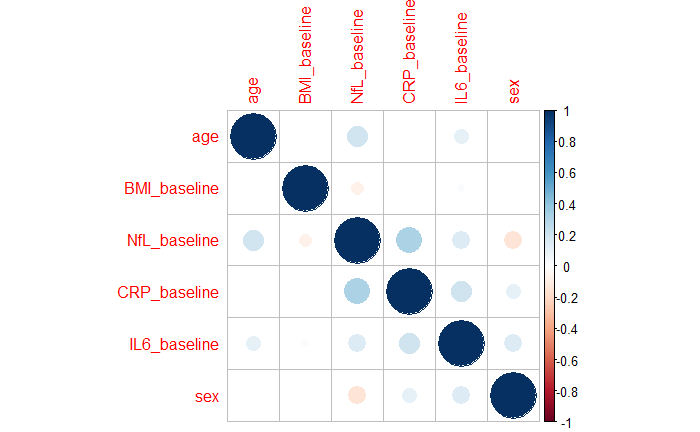
\includegraphics[width=0.6\textwidth]{corrplot.png} 
\caption{Matriz de correlación entre las variables predictoras. Los círculos más grandes indican correlaciones más fuertes.}
\label{fig:corrplot}
\end{figure}

De acuerdo con el análisis, la correlación más relevante se observa entre Nf-L y CRP, aunque sigue siendo moderada, lo que confirma que no existe una multicolinealidad problemática en el conjunto de variables consideradas.

\subsection{Selección de variables mediante algoritmo paso a paso y AIC}

Para optimizar la selección de predictores y minimizar el \emph{Akaike Information Criterion} (AIC), se aplicó el algoritmo paso a paso (\texttt{stepwise}) al modelo OLS previamente ajustado. Este procedimiento permitió eliminar variables que aportaban poca información explicativa, manteniendo únicamente aquellas que contribuyen significativamente a la predicción de la puntuación ALSFRS-R.

El modelo final seleccionado incluye únicamente las variables \texttt{onset} y \texttt{NfL\_baseline}, con los coeficientes mostrados en la Tabla~\ref{tab:stepwise}.

\begin{table}[h!]
\centering
\caption{Coeficientes del modelo final seleccionado por stepwise/AIC}
\label{tab:stepwise}
\begin{tabular}{lccc}
\hline
\textbf{Variable} & \textbf{Estimación} & \textbf{Error estándar} & \textbf{t-valor} \\
\hline
Intercept         & 43.742  & 1.735 & 25.207 \\
Onset (espinal)   & -2.908  & 1.589 & -1.830 \\
NfL\_baseline     & -0.023  & 0.005 & -4.391 \\
\hline
\end{tabular}
\end{table}

El coeficiente de \texttt{onset} indica que, en promedio, los pacientes con inicio espinal presentan puntuaciones ALSFRS-R más bajas. El coeficiente de \texttt{NfL\_baseline} también es negativo, indicando que mayores niveles de Nf-L se asocian con puntuaciones funcionales menores.

El modelo final explica aproximadamente el 17.3\% de la variabilidad en ALSFRS-R (\(R^2 = 0.1734\)), con un p-valor del modelo global muy significativo (\(p = 0.0001565\)), confirmando que los predictores seleccionados aportan información relevante para la predicción de la puntuación funcional.

Este resultado coincide con los análisis previos, que identificaron a Nf-L y al sitio de inicio como variables con una alta capacidad predictiva en la puntuación ALSFRS-R.

\subsection{Modelo PLS y detección de outliers}

Para explorar la capacidad predictiva de las variables y reducir la dimensionalidad, se ajustó un modelo de regresión \emph{Partial Least Squares} (PLS) sobre la puntuación ALSFRS-R, considerando las mismas variables regresoras utilizadas en el modelo OLS. El número óptimo de componentes se determinó a partir de los valores de \emph{Root Mean Square Error of Prediction} (RMSE) obtenidos mediante validación cruzada.

\begin{figure}[h!]
\centering
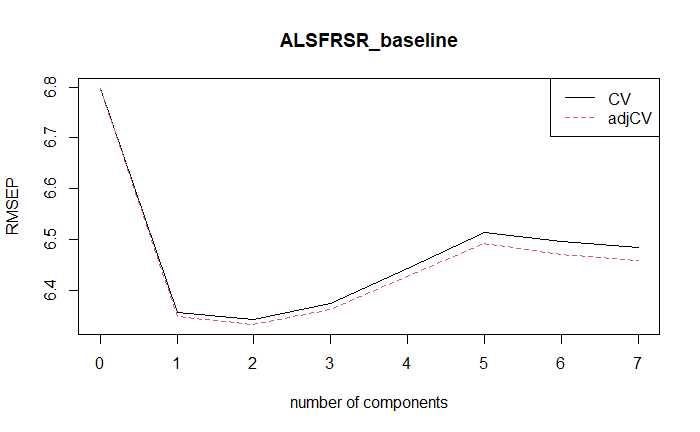
\includegraphics[width=0.6\textwidth]{RMSEP_plot_placeholder.png}
\caption{Evolución del RMSE según el número de componentes en el modelo PLS.}
\label{fig:pls_rmse}
\end{figure}

Como se observa en la Figura~\ref{fig:pls_rmse}, la reducción del RMSE se estabiliza a partir de dos componentes. Por tanto, se seleccionaron las dos primeras componentes como las más razonables para el modelo.

Con el objetivo de detectar posibles valores extremos o sesgos, se representó un diagrama de dispersión de los scores de las dos primeras componentes principales (Figura~\ref{fig:pls_scores}). Los sujetos alejados de la nube principal se consideran outliers potenciales.

\begin{figure}[h!]
\centering
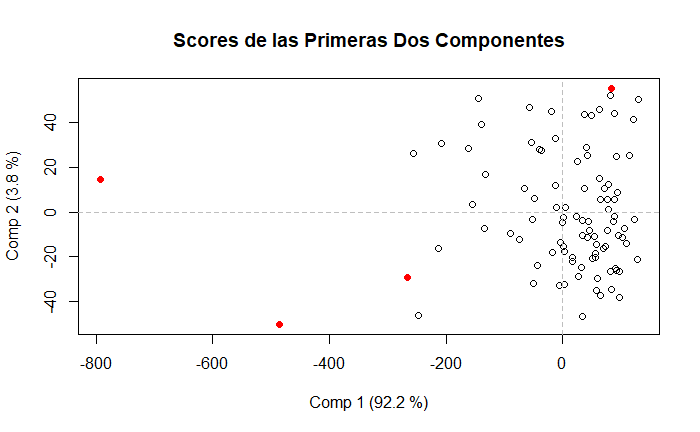
\includegraphics[width=0.6\textwidth]{PLS_scores_plot_placeholder.png}
\caption{Diagrama de dispersión de los scores de las dos primeras componentes principales del modelo PLS. Los puntos rojos indican sujetos potencialmente atípicos.}
\label{fig:pls_scores}
\end{figure}

Mediante un criterio basado en la desviación estándar de los scores, se identificaron cuatro sujetos como outliers: 17, 26, 734 y 737. Estos pacientes presentan valores extremos en al menos una de las dos primeras componentes principales, lo que sugiere que podrían tener características atípicas en relación con el conjunto de predictores utilizados.

El análisis PLS permite, por tanto, seleccionar un número reducido de componentes explicativas y detectar sujetos con influencia especial en la predicción de la puntuación ALSFRS-R.

\subsection{Regresión LASSO}

Para evaluar la capacidad predictiva de un conjunto reducido de variables y obtener un modelo regularizado, se ajustó un modelo de regresión LASSO utilizando las variables: BMI\_baseline, IL6\_baseline, NfL\_baseline y CRP\_baseline como predictores de la puntuación ALSFRS-R.  

La selección de las variables se realizó mediante validación cruzada para determinar el valor óptimo de \(\lambda\) que minimiza el error de predicción (\(\lambda_{\min}\)). A partir de este valor, se obtuvieron los coeficientes del modelo.  

Los coeficientes correspondientes a \(\lambda_{\min}\) fueron los siguientes:

\begin{table}[h!]
\centering
\begin{tabular}{lrr}
\hline
Variable & Coeficiente \\ \hline
Intercepto & 39.4687 \\
BMI\_baseline & 0 \\
IL6\_baseline & 0.0286 \\
NfL\_baseline & -0.0179 \\
CRP\_baseline & 0 \\ \hline
\end{tabular}
\caption{Coeficientes del modelo LASSO para \(\lambda_{\min}\).}
\label{tab:lasso_coef}
\end{table}

A partir de estos coeficientes, la fórmula del modelo LASSO se puede expresar como:

\[
\text{ALSFRSR\_baseline} = 39.4687 + 0.0286 \cdot \text{IL6\_baseline} - 0.0179 \cdot \text{NfL\_baseline}
\]

Observamos que dos de las cuatro variables seleccionadas (BMI\_baseline y CRP\_baseline) fueron eliminadas por el procedimiento de penalización, quedando únicamente IL6\_baseline y NfL\_baseline como predictores activos. Esto indica que el modelo regularizado selecciona las variables más informativas y reduce la complejidad del ajuste.

\subsection{Comparación de RMSE entre los diferentes modelos}

Para evaluar qué método proporciona el mejor ajuste predictivo de la puntuación ALSFRS-R, se calcularon las predicciones de los modelos OLS, Stepwise, PLS y LASSO sobre la cohorte de validación ValCohort2. A partir de estas predicciones, se calculó el \emph{Root Mean Squared Error} (RMSE) para cada modelo:

\begin{table}[h!]
\centering
\begin{tabular}{lc}
\hline
Modelo & RMSE \\ \hline
OLS & 5.5981 \\
Stepwise & 5.5430 \\
PLS & 5.3632 \\
LASSO & 5.2072 \\ \hline
\end{tabular}
\caption{RMSE de los distintos modelos en la cohorte ValCohort2.}
\label{tab:rmse_models}
\end{table}

De los resultados, se observa que el modelo LASSO alcanza el menor RMSE, indicando que tiene la mejor capacidad predictiva sobre ValCohort2. Esto sugiere que, entre los métodos evaluados, LASSO es el más eficiente para predecir la puntuación ALSFRS-R, al minimizar el error cuadrático medio frente a los valores reales de la cohorte de validación.














\begin{thebibliography}{9}

\bibitem{Witzel2021} S. Witzel, et al. (2021). \textit{Neurofilament light and heterogeneity of disease progression in amyotrophic lateral sclerosis: development and validation of a prediction model to improve interventional trials}. Translational Neurodegeneration.

\end{thebibliography}
\end{document}